\documentclass{sig-alternate}

\makeatletter
 \let\@copyrightspace\relax
 \makeatother

\usepackage{CJKutf8}
\usepackage{graphicx}
\usepackage{makeidx}  % allows for indexgeneration
\usepackage{amsmath}
\usepackage{bm}
\usepackage{multirow}

\begin{document}

\title{Nders at NTCIR-13 Short Text Conversation 2 Task}

\numberofauthors{3} %  in this sample file, there are a *total* of EIGHT authors.
\author{
% You can go ahead and credit any number of authors here,
% e.g. one 'row of three' or two rows (consisting of one row of three
% and a second row of one, two or three).
%
% The command \alignauthor (no curly braces needed) should
% precede each author name, affiliation/snail-mail address and
% e-mail address. Additionally, tag each line of
% affiliation/address with \affaddr, and tag the
% e-mail address with \email.
%
% 1st. author
\alignauthor
Han Ni\\
       \affaddr{NetDragon Websoft Inc., China}\\
       \email{nihan@nd.com.cn}
% 2nd. author
\alignauthor
Liansheng Lin\\
       \affaddr{NetDragon Websoft Inc., China}\\
       \affaddr{Fuzhou University, China}\\
       \email{linliansheng@nd.com.cn}
% 3rd. author
\alignauthor 
Ge Xu\\
       \affaddr{Minjiang University, China}\\
       \email{XuGeNLP@nd.com.cn}
}



\maketitle

\begin{abstract}
This paper describes our retrieval-based approaches at NTCIR-13 short text conversation 2 
(STC-2) task (Chinese). For a new post, our system firstly retrieves similar posts 
in the repository and gets their corresponding comments, and then finds the 
related comments directly from the repository. Moreover, we devise two new methods. 1)  LSTM-Sen2Vec model to get the vector of sentence. 2) Pattern-IDF 
to rerank the candidates from above. Our best run achieves 0.4780 for mean nG@1, 
0.5497 for mean P+, and 0.5882 for mean nERR@10, and respectively rankes 4th, 
5th, 5th among 22 teams. 
\end{abstract}

\section*{Team Name}
Nders

\section*{Subtasks}
Short Text Conversation 2 (Chinese)

\keywords{Short Text Conversation, LSA, LDA, Word2Vec, LSTM, Pattern-IDF, Sen2Vec}

\section{Introduction}

We participated in the NTCIR-13 Short Text Conversation 2 (STC-2) Chinese 
subtask. Given a new post, this task aims to retrieve an appropriate comment 
from a large post-comment repository (Retrieval-based method) or generate a new 
appropriate comment (Generation-based method). Our system chooses the 
retrieval-based method. 

The retrieved or generated comment for the new post is judged from four 
criteria: Coherent, Topically relevant, Non-repetitive and Context 
independent\cite{Lifeng}\cite{Lifeng-13}. The primary criterion for a suitable comment we consider is 
topically relevant. In other words, this comment should be talking about the 
same topic with the given post. We train LSA\cite{Susan} model and LDA\cite{David} 
model to obtain the degree of topic relateness, Word2Vec\cite{Mikolov} model 
to obtain the semantic similarity between new post and retrieved comment. 
By combining them together, we proposed a simialrity score to search comment 
candidates, and achieves a good performance.

Based on a hypothesis, similar posts has similar corresponding comments, we try 
to find the similar posts to the new post and get their corresponding comments 
as a supplement for the candidates. In addition to Word2Vec model and LSA model, 
we also introduce Sen2Vec model trained by LSTM\cite{Hoch}\cite{Martin}\cite{{Graves}} to compute similarity between two sentences.

In the last step, we rank the candidates by TextRank and Pattern-IDF. Results 
show that Pattern-IDF improves the performance while TextRank deteriorates it 
instead.

The remainder of this paper is organized as follows: Section 2 describes our 
systems in detail. Our experimental results are presented in Section 3. 
We make conclusions in Section 4.

\section{System Architecture}
The architecture of our system is described as Figure 1. 

\begin{figure}
  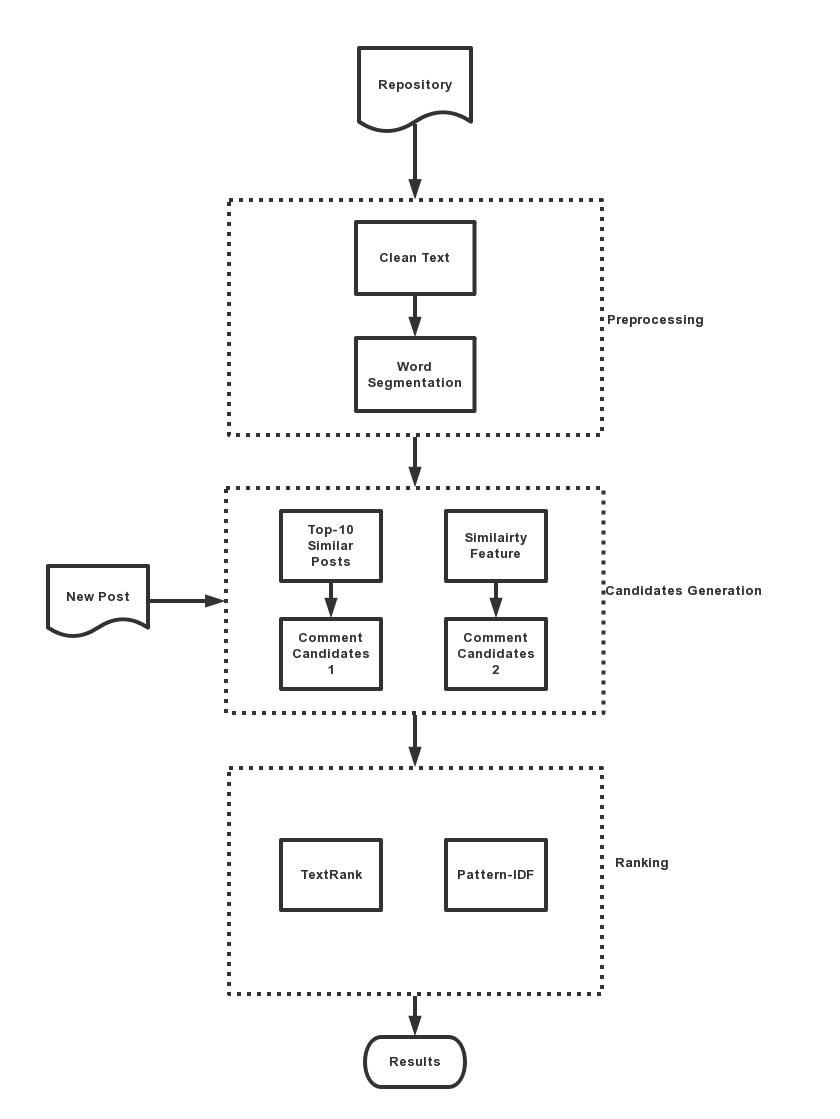
\includegraphics[height=4.6in, width=3.3in]{stc-flow.png}
  \caption{System Architecture}
\end{figure}

\subsection{Preprocessing}
There are some traditional Chinese in raw text which will cause incorrect 
word segmentation, so we convert traditional Chinese to simplified Chinese with 
nstools\footnotemark.\ Moreover, we convert full-width characters into half-width
ones. In addition, we replace all the number, datetime, url with token \emph{<\_NUM>}, 
\emph{<\_TIME>}, \emph{<\_URL>} respectively.
\footnotetext{https://github.com/skydark/nstools}

Unlike English words in a sentence are separated by spaces, Chinese short texts 
are written without any symbol between characters. So the word segmentation 
becomes necessary. We choose nlpir\footnotemark\ to segment the chinese text. 
After segmentation, our system filters meaningless words and symbols according 
to Chinese stop words list in order to clean the result.

The following example in Table 1 shows the raw text, segmentation result 
without and with traditional-simplified conversion (T-S conversion for short), 
and clean result.

\begin{table*}
\centering
\caption{The preprocessing result}
\begin{tabular}{l@{\qquad}l}
\hline\noalign{\smallskip}
Short Text ID & test-post-10440 \\
\noalign{\smallskip}
\hline
\noalign{\smallskip}
Raw Text          & \begin{CJK}{UTF8}{bsmi}去到美國,\begin{CJK}{UTF8}{gbsn}还\end{CJK}是吃中餐!宮保雞丁家的感覺~\end{CJK}  \\
\hline
\noalign{\smallskip}
Without T-S Conversion  & \begin{CJK}{UTF8}{bsmi}去 到 美 國 , \begin{CJK}{UTF8}{gbsn}还\end{CJK} 是 吃 中餐 ! 宮 保 雞 丁 家 的 感 覺 \end{CJK} \~{} \\
\hline
\noalign{\smallskip}
With T-S Conversion   & \begin{CJK}{UTF8}{gbsn}去 到 美国 , 还 是 吃 中餐 ! 宫保鸡丁 家 的 感觉 \~{}\end{CJK}   \\
\hline
\noalign{\smallskip}
Clean Result   & \begin{CJK}{UTF8}{gbsn}去 到 美国 还 是 吃 中餐 宫保鸡丁 家 的 感觉\end{CJK}   \\
\hline
\end{tabular}
\end{table*}

\footnotetext{http://ictclas.nlpir.org/}

\subsection{Similarity Features}
In order to compute the degree of similarity or relateness between two 
sentences, we convert text sentence into continuous vector representations 
with some techniques including LSA, LDA, Word2Vec, LSTM-Sen2Vec. While not 
using TF-IDF as the similarity feature directly, it would participate in 
training LDA, LSA models and calculate the similarity score by using Word2Vec, see 2.2.5.

\subsubsection{TF-IDF}
In information retrieval, TF-IDF, short for term frequency – inverse document frequency, is a numerical statistic that is intended to reflect how important a word is to a document in a collection or corpus. It is often used as a weighting factor in information retrieval, text mining, and user modeling. 

TF-IDF is the product of two statistics, term frequency and inverse document frequency. Various ways for determining the exact values of both statistics exist.

In the case of the term frequency $TF(t,d)$, the simplest choice is to use the raw count of a term in a document, i.e. the number of times that term $t$ 
occurs in document $d$. 

The inverse document frequency is a measure of how much information the word provides, that is, whether the term is common or rare across all documents. It is the logarithmically scaled inverse fraction of the documents that contain the word, obtained by dividing the total number of documents by the number of documents containing the term, and then taking the logarithm of that quotient.

\begin{equation}
IDF(t, D) = \log{\frac{N}{|{d \in D: t \in d}|}}
\end{equation}
Where, $N$ refers to the total number of documents in the corpus, $N = |D|$. $|{d \in D: t \in d}|$ refers to the number of documents where the term $t$ appears. If the term is not in the corpus, this will lead to a division-by-zero. It is therefore common to adjust the denominator to $1 + |{d \in D: t \in d}|$.

Then, TF-IDF is calculated as
\begin{equation}
TF-IDF(t,d,D) = TF(t,d) \cdot IDF(t, D)
\end{equation}

\subsubsection{LSA}
Latent semantic analysis (LSA) is a technique of analyzing relationships between a set of documents and the terms they contain by producing a set of concepts related to the documents and terms. LSA assumes that words that are close in meaning will occur in similar pieces of text (the distributional hypothesis). A matrix containing word counts per paragraph (rows represent unique words and columns represent each paragraph) is constructed from a large piece of text and a mathematical technique called singular value decomposition (SVD) is used to reduce the number of rows while preserving the similarity structure among columns.\cite{Susan} We combine each post with its corresponding comments to be a document, then we train LSA model (200 topics) on these documents with gensim\footnotemark. From trained model, we can get vector for each chinese word.
Then, we can get vector representation of a sentence by Eq.3:
\begin{equation}
   V = \frac{1}{n} \cdot \sum_{i=1}^n v_i 
\end{equation}
Here, capital $V$ refers to vector of a sentence, $v_i$ refers to vector of each word in the sentence, and $n$ is the length of the sentence.

\footnotetext{https://radimrehurek.com/gensim/index.html}

\subsubsection{LDA}
Latent Dirichlet allocation (LDA) is a generative statistical model that allows sets of observations to be explained by unobserved groups that explain why some parts of the data are similar. For example, if observations are words collected into documents, it posits that each document is a mixture of a small number of topics and that each word's creation is attributable to one of the document's topics.\cite{David} Like training LSA model, we combine each post with its corresponding comments to be a document, then we train LDA model (200 topics) on these documents with gensim. With trained LDA model, we can transform new, unseen documents into LDA topic distributions. We regard a sentence(a post, or a comment) as a document, convert it into plain bag-of-words count vector, and then index LDA model to obtain a vector representation of the sentence. 

\subsubsection{Cosine Similarity} 
After convert sentence into vectors, we compute similarity of two sentences by cosine similarity:
\begin{equation}
   Sim(s_1, s_2) = \frac{V_1 \cdot V_2}{\left \| V_1 \right \| \left \| V_2 \right \|}
\end{equation}
Here, $V_1$ refers to vector representation of sentence $s_1$, $V_2$ refers to vector representation of sentence $s_2$.

With sentence vectors from different models, we get corresponding sentence similarity. We use $Sim_{LSA}$ to denote sentence similarity based on LSA model, and $Sim_{LDA}$ to denote sentence similarity based on LDA model.

\subsubsection{Word2Vec}
Word2Vec is an efficient tool for computing continuous distributed 
representations of words\cite{Mikolov}. We train our Word2Vec model on provided 
post-comment pairs in repository and training 
data with skip-gram architecture where window size is 7, vector 
length is 300 and min count is 5 to remove infrequent words. Vector 
representation for each chinese word is directly obtained from trained model. 

Moreover, when using Word2Vec to calculate the sentence vector, we normalize every 
word's norm to its corresponding square root of value of IDF. Sum all words within a sentence and divede by its length, as below:

\begin{equation}
   V = \frac{1}{n} \cdot \sum_{i=1}^n v_i \cdot \frac{\sqrt{IDF(w_i)}}{|v_i|} 
\end{equation}
Here, capital $V$ refers to vector of a sentence, $v_i$ refers to vector of each word $w_i$ in the sentence, $IDF(w_i)$ refers to inverse document frequence for word $w_i$, and $n$ is the length of the sentence.

Then, we calculate Word2Vec similarity by Eq.4, denoted as $Sim_{W2V}$.

\subsubsection{LSTM-Sen2Vec}
Word2Vec, LDA and LSA models capture the word meaning by the word distribution 
of its context, which ignores the order of words in a sentence. To take the order 
into account, we design a new model which can calculate the sentence vector 
with the sequence information, we call it LSTM-Sen2Vec.

Long short-term memory (LSTM) is a recurrent neural network (RNN) architecture 
that remembers values over arbitrary intervals. Figure 2 shows the architecture 
of LSTM. The $C_t$ represents the cell state at time $t$ and it is stored as a 
vector, which can theoretically remember all the previous information. The 
$h_t$ represents current hidden state, which is also a output value at time 
$t$. The following equations describe the details of the architecture:
\begin{equation}
   f_t = \sigma(W_f \cdot [h_{t-1}, x_t] + b_f)
\end{equation}
\begin{equation}
   i_t = \sigma(W_i \cdot [h_{t-1}, x_t] + b_i)
\end{equation}
\begin{equation}
   \tilde{C}_t = tanh(W_C \cdot [h_{t-1}, x_t] + b_C) 
\end{equation}
\begin{equation}
   C_t = f_t * C_{t-1} + i_t * \tilde{C}_t
\end{equation}
\begin{equation}
   o_t = \sigma(W_o \cdot [h_{t-1}, x_t] + b_o)
\end{equation}
\begin{equation}
   h_t = o_t * tanh(C_t)
\end{equation}
Where $W_f, W_i, W_c, W_o, b_f, b_i, b_c, b_o$ refer to corresponding weights and bias.
\begin{figure}
  \centering
  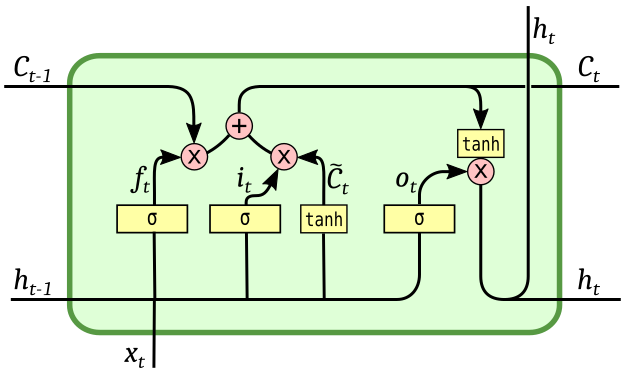
\includegraphics[height=1.5in, width=2.44in]{lstm2.png}
  \caption{The repeating module in an LSTM contains four interacting layers.}
\end{figure}

Mikolov\cite{Mikolov2} and Zaremba\cite{Zaremba} use LSTM to predict the next 
word given the previous words as input and achieve a good perplexity. Inspired 
by their architecture of LSTM, we can use the vector of the final cell state to 
represent a sentence by feeding its words as input in sequence.

We train the model using unidirectional LSTM, whose architecture is shown as 
Figure 3. 

Before training the LSTM model, we train the Word2Vec model as its word embedding 
vector and freeze it while the whole training process. The hidden size of LSTM 
cell is 300 which is the same as Word2Vec’s dimension, and the total layers
are 3, the forget bias is set to 1.0, with SGD as the optimizer and 0.95 decay 
every 2 epochs. 

For a new post, we calculate its 
similarity with other post by the value of cosine similarity. When observe 
the result, we find that in the top-N similar posts, the last few words are 
extremely similar. Which suggests that the unidirectional LSTM 
model may assign much more weight to the end of a sentence. 

\begin{figure}
  \centering
  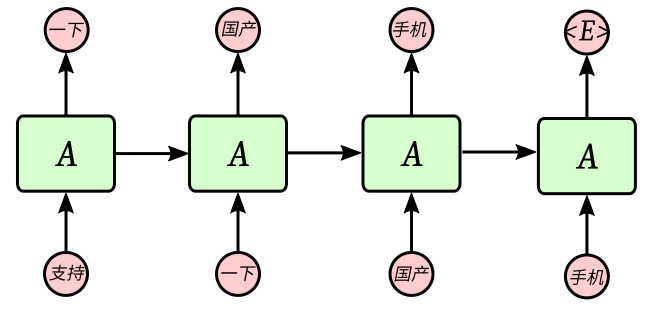
\includegraphics[height=1.5in, width=3.15in]{unilstm.png}
  \caption{The unidirectional LSTM}{We append an end token \emph{<E>} in the end of word sequence to fix the length of input and output}
\end{figure}

To overcome the unbalance, we replace unidirectional LSTM with bidirectional 
LSTM. The traditional bidirectional LSTM architecture is shown as Figure 4.
However, it doesn’t make sense if we concatenate the outputs of forward and 
backward at the same time step , because at each time step both of them
predict different words given the same word (such as “\begin{CJK}{UTF8}{gbsn}国产\end{CJK}” concatenated with “\begin{CJK}{UTF8}{gbsn}支持\end{CJK}”, shown as Figure 4).

\begin{figure}
  \centering
  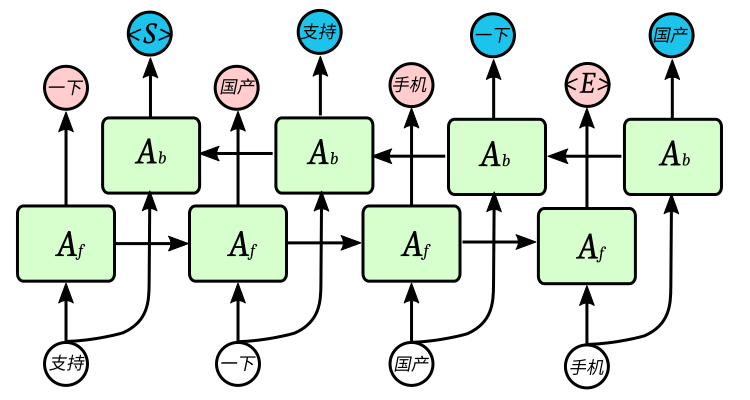
\includegraphics[height=1.5in, width=2.81in]{bilstm1.png}
  \caption{The Traditional Bidirectional LSTM}
\end{figure}

\begin{table}
\centering
\caption{Word-level perplexity on the Penn Tree Bank Dataset}
\label{tab:commands}
\begin{minipage}{\columnwidth}
\begin{center}
\begin{tabular}{c c c}
\hline
         &   Validation set &  Test set   \\ \hline
 Unidirectional LSTM & 71.9 & 68.7 \\ \hline
 Modified Bidirectional LSTM & 68.4 & 66.9 \\ \hline
\end{tabular}
\end{center}
\end{minipage}
\end{table}

So we modify to make the concatenation rational, shown as Figure 5. 
Then we concatenate the outputs of both directions at each time step, which 
is 600-dimension. Through a full connection layer, it is reduced to 
dimension 300. We calculate the Euclidean distance of each output and its 
vector of Word2Vec model as the cost of neural networks. The word-level perplexity of our model on the Penn Tree Bank Dataset is shown as Table 2.

\begin{figure*}
  \centering
  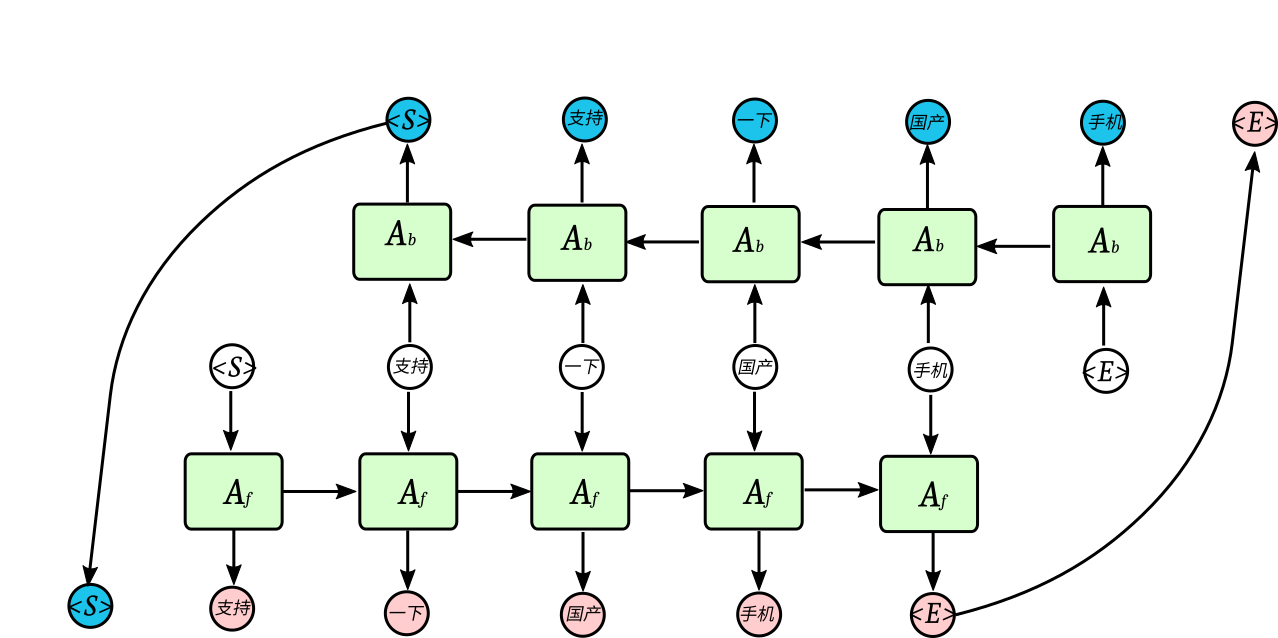
\includegraphics[height=3in, width=6.21in]{bilstm2.png}
  \caption{The Modified Bidirectional LSTM}{In order to align the outputs of forward and backward direction, we append the first output value (indicates start token \emph{<S>}) of  
  backward direction to the outputs of forward, and append the last output value (indicates end token \emph{<E>}) of forward direction to the outputs of backward.}
\end{figure*}

Finally, we concatenate the final cell states of two direction as the vector of 
the input sentence which is 600-dimension.

\subsection{Candidates Generation}

\subsubsection{Similar Posts}
Based on a hypothesis that similar posts has similar corresponding comments, we firstly find top-10 similar posts with a ranking score combining LSA, Word2Vec, and LSTM model:
\begin{equation}
   Score_{q,p}(q, p) = Sim_{LSA}(q, p) * Sim_{W2V}(q, p) * Sim_{LSTM}(q, p)
\end{equation}
Here, $q$ denotes the query(the new post) $p$ denote the post from repository.

Then, we get corresponding comments to the top-10 similar posts as first comment candidates, denoted as $C_1$.

\subsubsection{Comment Candidates}
Since Word2Vec model captures semantic similarity, LSA or LDA reflects topic relateness, we combine LSA or LDA with Word2Vec respectively to directly retrieve top-N appropriate comments to the new post from all comments in the repository. N is equal to the number of comment candidates $C_1$. 
\begin{equation}
   Score_{q,c}^1(q, c) = Sim_{LSA}(q, c) * Sim_{W2V}(q, c)
\end{equation}
\begin{equation}
   Score_{q,c}^2(q, c) = Sim_{LDA}(q, c) * Sim_{W2V}(q, c)
\end{equation}
Here, $q$ denotes the query(the new post), $c$ denotes the comment from repository.

We combine the retrived top-N comments by Word2Vec model and LSA (or LDA) model with $C_1$ as final comment candidats for further ranking.

\subsection{Ranking}

\subsubsection{TextRank}

TextRank\cite{Mihalcea} is a graph-bsed ranking model for text processing. 
Graph-based ranking algorithms are essentially a
way of deciding the importance of a vertex within
a graph, based on global information recursively
drawn from the entire graph. The basic idea implemented
by a graph-based ranking model is that
of voting or recommendation. When one vertex
links to another one, it is basically casting a vote
for that other vertex. The higher the number of votes
that are cast for a vertex, the higher the importance
of the vertex. Moreover, the importance of the vertex
casting the vote determines how important the vote
itself is, and this information is also taken into account
by the ranking model. Hence, the score associated
with a vertex is determined based on the votes
that are cast for it, and the score of the vertices casting
these votes.

We consider an undirected weighted TextRank algorithm in our system. 
Formally, let $G = (V, E)$ be a undirected graph with the set of vertices $V$ and 
and set of edges E, where E is a subset of $V \times V$. For a given $V_i$, let 
$link(V_i)$ be the set of vertices that linked with it. The score of a vertex 
$V_i$ is define as follow:
\begin{equation}
  WS(V_i) = (1 - d) + d * \sum_{j \in link(V_i)}{w_{ij} * WS(V_j)}
\end{equation}
where $d$ is a damping factor\cite {Brin} that is usually set to 0.85.

We add each unique word in candidates as a vertex in the graph and use a 
co-occurrence relation as edges between vertices in the graph. The edge is 
weighted by word2vec similarity between two words and the number of their 
co-occurrence. Here co-occurrence means two words co-occur within a window of 
maximum $W$ words, where the window size $W$ is set to be 5 in our system.

In our system, the TextRank value for each vertex refers to the importance of 
the word in candidates. We compute the TextRank value iteratively.

Firstly, for comment candidates, we create a dictionary $D$, a mapping between words 
and their integer ids. Such that, each unique word is mapped to a integer range 
from $0$ to $k-1$, $k$ is the size of the dictionary. We use $D_i$ to denote a 
word whose id is $i$.

Therefore, the $w_{ij}$ is defined as
\begin{equation}
  w_{ij} = cnt * Sim(D_i, D_j)
\end{equation}
When we scan the candidates sentence by sentence, if the word $D_i$ and $D_j$ 
co-occur within the window, the count for them increases by 1. The $cnt$ in Eq.16
refers to the total count after scanning.

Then, we construct a $k \times k$ matrix $\bm{M}$, defined as
\begin{equation}
  \begin{aligned}
    M_{ij} = \begin{cases} 
             w_{ij} & j \in link(D_i) \\
             0 & otherwise
             \end{cases}
  \end{aligned}
\end{equation}

At time t = 0, We initiate a $k$-dimension vector $\bm{R}$, where each entry is defined as the inverse document frequency (IDF) of the word: 
\begin{equation}
  R_i = IDF(D_i)
\end{equation}

At each time step, the computation yields:
\begin{equation}
  \bm{R(t+1)} = d\bm{M}\bm{R(t)} + \frac{1-d}{k} \bm{1}
\end{equation}

The computation ends when for some small $\epsilon$, $|\bm{R(t+1)} - \bm{R(t)} < \epsilon|$, Where we set $\epsilon = 10^{-7}$.

Since we get the score $R(D_i)$ for each word $D_i$, the score for each comment candidate $c$ is calculated as:
\begin{equation}
  Rank_{TextRank}(c) = \frac{\sum_{D_i \in c}{R(D_i)}}{len(c)} 
\end{equation}
where, $len(c)$ refers to the number of words in comment $c$.

Finally, we use $Rank_{TextRank}$ to rank the comment candidates and get top-10 comments as our Nders-C-R3 results for each given new post.

\subsubsection{Pattern-IDF}
Consider the hypothesis, similar posts have similar corresponding comments. In 
other words, for the corresponding comments of similar posts, the word 
distribution may also be similar. Therefore, we can use word distribution of 
the corresponding comments of post in the repository to infer that of the new post. We present a new model, Pattern-IDF (PI).

For word $D_i$ in corresponding comment given word $D_j$ in post, we define PI as:
\begin{equation}
  PI(D_i|D_j) = 1 / \log_{2}{\frac{count_c(D_i) * count_p(D_j)}{count_{pair}(D_i, D_j) + 1}}
\end{equation}
Here $count_c$ refers to the number of occurrence in comments, $count_p$ in posts, $count_{pair}$ in post-comment pair.

Table 2 shows some example of Pattern-IDF.
\begin{table}[]
\centering
\caption{The example of Pattern-IDF}
\label{my-label}
\begin{tabular}{lll}
\hline
 $D_j$ & $D_i$ & PI \\ \hline
 \begin{CJK}{UTF8}{gbsn}中国移动\end{CJK} & \begin{CJK}{UTF8}{gbsn}接通\end{CJK}   & 0.071725 \\ \hline
 \begin{CJK}{UTF8}{gbsn}中国移动\end{CJK} & cmcc                                  & 0.067261 \\ \hline
 \begin{CJK}{UTF8}{gbsn}中国移动\end{CJK} & \begin{CJK}{UTF8}{gbsn}资费\end{CJK}   & 0.062408 \\ \hline
 \begin{CJK}{UTF8}{gbsn}中国移动\end{CJK} & \begin{CJK}{UTF8}{gbsn}营业厅\end{CJK} & 0.059949 \\ \hline
 \begin{CJK}{UTF8}{gbsn}中国移动\end{CJK} & \begin{CJK}{UTF8}{gbsn}漫游\end{CJK}   & 0.059234 \\ \hline
 ... & ...  & ...  \\ \hline
 \begin{CJK}{UTF8}{gbsn}中国移动\end{CJK} & \begin{CJK}{UTF8}{gbsn}我\end{CJK}    & 0.028889 \\ \hline
 \begin{CJK}{UTF8}{gbsn}中国移动\end{CJK} & \begin{CJK}{UTF8}{gbsn}是\end{CJK}    & 0.027642 \\ \hline
 \begin{CJK}{UTF8}{gbsn}中国移动\end{CJK} & \begin{CJK}{UTF8}{gbsn}的\end{CJK}    & 0.026346 \\ \hline
\end{tabular}
\end{table}


For each comment $c$ in candidates, given a query (new post) $q$, we calculate the score by Pattern-IDF as follow:
\begin{equation}
  Score_{PI}(q, c) = \frac{\sum_{D_j \in q}{\sum_{D_i \in c}{PI(D_i|D_j)}}}{len(c) * len(q)}
\end{equation}

Then we define rank score as follow:
\begin{equation}
  Rank_{PI} = (1 + Score_{PI}(q, c)) * Sim_{W2V}(q, c)*Sim_{LSA}(q, c)  
\end{equation}

Finally, we use $Rank_{PI}$ to rank the comment candidates and get top-10 comments as our Nders-C-R2 results for each given new post.

\subsubsection{TextRank + Pattern-IDF}
In this method, We add each comment sentence in candidates as a vertex in the 
graph and use Word2Vec similarity as edges between vertices in the graph. 

At time t = 0, We initiate a $l$-dimension vector $\bm{P}$, here $l$ is the 
number of comment candidates. And each entry of $\bm{P}$ is defined as the 
score of Pattern-IDF between the query (new post) $q$ and corresponding comment
$c_i$ in candidates:
\begin{equation}
  P_i = Score_{PI}(q, c_i)
\end{equation} 

Then, we construct a $l \times l$ matrix $\bm{M}$, defined as
\begin{equation}
  \begin{aligned}
    M_{ij} = Sim_{W2V}(c_i, c_j)
  \end{aligned}
\end{equation}

At each time step, the computation yields:
\begin{equation}
  \bm{P(t+1)} = d\bm{M}\bm{P(t)} + \frac{1-d}{l} \bm{1}
\end{equation}

The computation ends when for some small $\epsilon$, $|\bm{P(t+1)} - \bm{P(t)} < \epsilon|$, Where we set $\epsilon = 10^{-7}$.

Finally, we get the score $P_i$ for each comment in candidates. After sorting, 
the top-10 comments are obtained as our Nders-C-R2 results.

\section{Experiments}

\subsection{Data Set}
Table 4 shows the statistics of the retrieval repository, training
data and test data. There are 219,174 Weibo posts and the
corresponding 4,305,706 comments. There are 4,433,949 post-comment
pairs. So each post has 20 different comments on
average, and one comment can be used to respond to multiple
different posts. 

There are 769 query posts in training data, each of which has about 15 
candidate comments. Totally, there are 11,535 comments labeled with 
\emph{suitable}, \emph{neutral}, and \emph{unsuitable}. \emph{Suitable} means that the comment 
is clearly a suitable comment to the post, \emph{neutral} means that the comment 
can be a comment to the post in a specific scenario, while \emph{unsuitable} means 
it is not the two former cases. 

100 query posts are used for test. Each team is permitted to submit five
runs to the task. In each run, a ranking list of ten comments for
each test query is requested. 

\begin{table}
\centering
\caption{Statistics of dataset for Chinese subtask}
\label{my-label}
\begin{minipage}{\columnwidth}
\begin{center}
\begin{tabular}{|l@{\quad}|l@{\quad}|@{\quad}r|}
\hline
\multirow{3}{*}{Repository}
                  & \#posts           & 219,174   \\ \cline{2-3} 
                  & \#comments        & 4,305,706 \\ \cline{2-3} 
                  & \#original pairs  & 4,433,949 \\ \hline
\multirow{3}{*}{Training Data} 
                  & \#posts           & 769       \\ \cline{2-3} 
                  & \#comments        & 11,535    \\ \cline{2-3} 
                  & \#labeled pairs   & 11,535    \\ \hline
Test Data         & \#query posts     & 100       \\ \hline
\end{tabular}
\end{center}
\end{minipage}
\end{table}

\subsection{Evaluation Measures}
Following the NTCIR-12 STC-1 Chinese subtask, three evaluation measures are
used: nG@1 (normalised gain at cut-off 1), P+, and nERR@10 (normalised expected reciprocal rank at cutoff 10)\cite{Lifeng}\cite{Lifeng-13}.

nG@1 shows the quantity of effective result in the retrieved candidates. 

P+ depends most on the position of the best effective result in the
ranking list of retrieved candidates. It gives the top ranked result
the most ratio. 

nERR@10 shows the rank correctness of the candidates ranking,
which means that the more effective result should be ranked as
more front of the ranking list of retrieved candidates.

\subsection{Experimental Results}
We submitted five runs for comparison and analysis:

\begin{enumerate}
  \item{Nders-C-R5: } Use $Sim_{W2V}*Sim_{LDA}$ as a ranking score to directly 
  retrieve and get top-10 comments from all comments.
  \item{Nders-C-R4: } Use $Sim_{W2V}*Sim_{LSA}$ as a ranking score to directly 
  retrieve and get top-10 comments from all comments.
  \item{Nders-C-R3: } Use graph-based algorithm TextRank with words as vertices
  in the graph, and use score $Rank_{TextRank}$ to rank comment in the 
  candidates and get top-10 comments.
  \item{Nders-C-R2: } Use $Rank_{PI}$ as a ranking score to get top-10 comments from comment candidates.
  \item{Nders-C-R1: } Use graph-based algorithm TextRank with comments as vertices in the graph and Pattern-IDF as initiate score for each comment to 
  rank the comment in the candidates and get top-10 comments.
\end{enumerate}

\begin{table}
\centering
\caption{The official results of five runs for Nders team}
\label{tab:commands}
\begin{minipage}{\columnwidth}
\begin{center}
\begin{tabular}{|l|c|c|c|}
\hline
 Run        &  Mean nG@1  &  Mean P+  &  Mean nERR@10  \\ \hline
 Nders-C-R1 & 0.4593 & 0.5394 & 0.5805 \\ \hline
 Nders-C-R2 & 0.4743 & \textbf{0.5497} & \textbf{0.5882} \\ \hline
 Nders-C-R3 & 0.4647 & 0.5317 & 0.5768 \\ \hline
 Nders-C-R4 & \textbf{0.4780} & 0.5338 & 0.5809 \\ \hline
 Nders-C-R5 & 0.4550 & 0.5495 & 0.5868 \\ \hline
\end{tabular}
\end{center}
\end{minipage}
\end{table}

The official results of our five runs are shown in Table 5. Which shows 
that, with the use of Word2Vec and LSA model, R4 achieves 
best result in our five runs for Mean nG@1, that ranks 4th among 22 teams. 

The best results in our runs for Mean P+ and Mean nERR@10 are both R2, 
which introduces Pattern-IDF to rank the comment candidates generated by 
Word2Vec and LSA model(R4). The result of R2 improves against R4 by $2.02\%$ for mean P+ and $1.26\%$ for mean nERR@10 and both ranks 5th among 22 teams, with $0.77\%$ slightly decreased for mean nG@1. It proves the 
effectiveness of the Pattern-IDF we devised. 

However, the results of R3 are worse than that of R4 for all three metrics, 
which shows TextRank is not helpful for candidates ranking in this task.

Compare the result of R4 and R5, we find that for Mean P+ and Mean nERR@10 the 
result of R5 is better than that of R4, which shows LDA model outperforms LSA 
model in this task.

\section{Conclusions}
In this paper, we propose an approach for STC-2 task of NTCIR-13. The LSA,
Word2Vec and LSTM-Sen2Vec model are used to find similar posts. The LSA and Word2Vec 
model are used to retrieve comment candidates. A graph-based algorithm TextRank 
and the Pattern-IDF we devised are applied to rank the candidates. Results show 
that the Pattern-IDF we devised is effective for ranking while TextRank not, 
and LDA model outperforms LSA model in retrieving candidates. Finally, our best 
run achieves 0.4780(R4) for mean nG@1, 0.5497(R2) for mean P+, and 0.5882(R2) for 
mean nERR@10, which respectively rankes 4th, 5th, 5th among 22 teams. 




%
% ---- Bibliography ----
%
\begin{thebibliography}{5}

\bibitem {Lifeng}
Lifeng Shang, Tetsuya Sakai, Zhengdong Lu, Hang Li, Ryuichiro Higashinaka, Yusuke Miyao. 
Overview of the NTCIR-12 Short Text Conversation Task, 2016.

\bibitem {Lifeng-13}
Lifeng Shang, Tetsuya Sakai, Hang Li, Ryuichiro Higashinaka, Yusuke Miyao, Yuki Arase, Masako Nomoto. 
Overview of the NTCIR-13 Short Text Conversation Task, 2017.

\bibitem {Susan}
Susan T. Dumais (2005). Latent Semantic Analysis. Annual Review of Information Science and Technology. 38: 188–230. 

\bibitem {David}
Blei, David M, A. Y. Ng, and M. I. Jordan. Latent dirichlet allocation. Journal of Machine Learning Research 3(2003):993-1022.

\bibitem {Mikolov}
Mikolov, Tomas, et al. Efficient Estimation of Word Representations in Vector Space. Computer Science (2013).

\bibitem {Mikolov2}
Mikolov, Toma's. Statistical Language Models Based on Neural Networks. Ph.D. thesis, Brno University of Technology.(2012)

\bibitem {Zaremba}
Zaremba, Wojciech, I. Sutskever, and O. Vinyals. Recurrent Neural Network Regularization. Eprint Arxiv (2014).

\bibitem {Hoch}
Hochreiter, S., \& Schmidhuber, J. (1997). Long short-term memory. Neural computation, 9(8), 1735-1780.

\bibitem {Martin}
Sundermeyer, Martin, R. Schlüter, and H. Ney. LSTM Neural Networks for Language Modeling. Interspeech 2012:601-608.

\bibitem {Graves}
Graves, Alex. Generating Sequences With Recurrent Neural Networks. Computer Science (2013).

\bibitem {Mihalcea}
Mihalcea, Rada, and P. Tarau. TextRank: Bringing Order into Texts. Unt Scholarly Works (2004):404-411.

\bibitem {Brin}
Brin, Sergey, and L. Page. The anatomy of a large-scale hypertextual Web search engine. International Conference on World Wide Web Elsevier Science Publishers B. V. 1998:107-117.


\end{thebibliography}

\end{document}

